\section{Using \tool{} as an Online Optimizer}
\label{sec:online}

Every time an optimization suggested by \tool{} in its offline
capacity is implemented, \tool{} loses some of its power to optimize
online.
%
Nevertheless, we feel it is worthwhile to evaluate \tool{} online,
though its power is less than it would have been a few years ago.


When using \tool{} as an online compiler, we restrict it to
synthesizing constants, since it should nearly always be a win to
replace a value at the LLVM level with a constant.
%
Replacing an LHS in LLVM with instructions from an \tool{} RHS
introduces several performance-related difficulties that we have not
yet solved.
%
First, as discussed in Section~\ref{sec:offline}, estimating
profitability is difficult, especially in the presence of LLVM's
arcane canonicalization rules.
%
Second, \tool{} abstracts away the fact that some of the values in a
LHS are likely to have uses not visible in the \tool{} IR\@.
%
These uses will prevent instructions on the LHS from being eliminated
and may therefore dramatically reduce the benefit that is realized by
applying a particular optimization.
%
Third, naïvely replacing an LHS with a RHS can break SSA, since it is
not necessarily the case that the inputs to an LHS dominate the root of
a DAG of \tool{} IR\@.
%
Of course, this can be fixed up, but the fix is not free since it
forces values to be computed on code paths where they previously were
not computed.
%
In summary, there are significant challenges in automatically and
profitably implementing arbitrary \tool-derived optimizations that we
leave for future work.


\paragraph{Experimental setup}

For the experiments reported in this paper, we used an Intel i7-5820K
(3.3\,GHz, six-core Haswell-E) with 16\,GB of RAM running Ubuntu
14.04.
%
We configured the processor to use performance mode and disabled turbo
mode to minimize dynamic frequency scaling effects.
%
For the solver we used a current snapshot of Z3 version 4.5.1.
%
We used our patched Klee that emits queries in the theory of
quantified bitvectors rather than the theory of arrays.
%
Whenever possible, we ran compilations using all cores.
%
However, actual benchmarks were run on a single core of an otherwise
quiescent machine.


\paragraph{Optimizing LLVM}

The LLVM-3.9 compiler and its Clang frontend are, together, nearly
three million lines of C++.
%
We compiled them using \tool{}; this took about 88 minutes with a cold
cache and 14 minutes with a warm cache.
%
At the end of compilation, Redis was using 362\,MB of RAM and its
database dump file was 149\,MB.
%
In contrast, compilation without \tool{} took 13 minutes.
%
In both cases, the compilation was in release mode (full optimization,
no debugging symbols) with assertions enabled.


The \tool{}-optimized \texttt{clang} binary, which contains all of the
LLVM internals, is 64.3\,MB, in contrast with the non-\tool{}
binary which is 67.2\,MB: a savings of 2.9\,MB\@.
%
A lot of the code size savings appears to come from proving that
assertions cannot fire; when assertions are disabled (turned into nops
using the preprocessor), the \tool-optimized Clang binary is only
about 600\,KB smaller than the non-\tool{} version.
%
When used to perform optimized compiles of C++ code, the
\tool-optimized Clang is 2\% slower than the default release build of
Clang.
%
We suspect, but cannot (yet) prove that we are running afoul of an
unlucky combination of optimization interactions, since it should not
be the case that replacing values with constants (and often small
constants like 0 and 1 that are easy to materialize) results in worse
code generation.


When the test suite for the \tool{}-optimized LLVM/Clang is run, 92
out of about 17,000 test cases fail.
%
For every one of these that we inspected, LLVM/Clang executed
undefined behavior, which we believe to be the root cause of the
failing test cases, with \tool{} simply exposing the problem.
%
Our belief is not yet backed up by strong evidence, but we plan to work
with the LLVM developers to eliminate the undefined behaviors, and see
if the failures then go away.
%
If they do not, the evidence points to a defect in \tool{} that
we have been otherwise unable to locate.
%
We noticed that all of the \tool{} optimizations that triggered test
case failures involved blockpcs.
%
The 2\%-slower Clang executable described in this section was compiled
by \tool{} in a mode that did not extract blockpcs.


\paragraph{Is \tool{} acceptably fast?}

\begin{figure}
  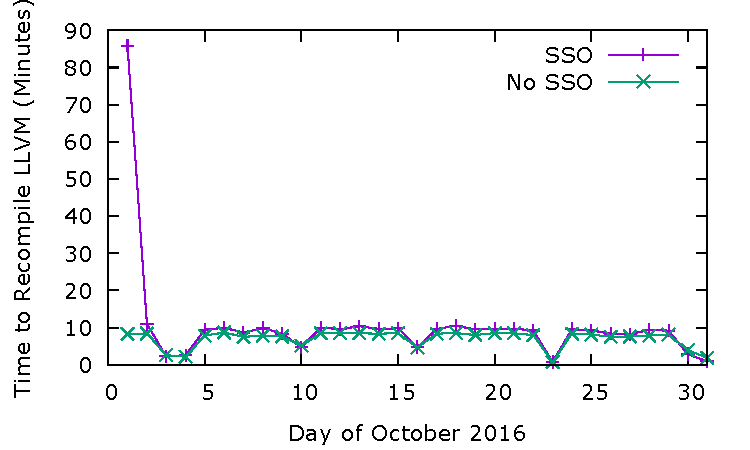
\includegraphics[width=\columnwidth]{figs/daily.pdf}
  \caption{Time taken to incrementally compile the LLVM development
    trunk at the start of each day of October 2016, with and without
  \tool{}.}
  \label{fig:daily}
\end{figure}

We simulated the experience a developer using \tool{} might have by
incrementally compiling LLVM (without Clang) from its development
trunk at the start of each day in October 2016.
%
Build times are shown in Figure~\ref{fig:daily}.
%
For a developer not using \tool{}, the first build took a little over
eight minutes, and so did most subsequent builds, because on most days
the LLVM developers checked in patches to one or more widely-included
header files, forcing a near-total recompilation.
%
On a few days, no such changes were committed and incremental
compilation was fast; it required less than one minute on October~23
and~31.


For the developer using \tool{}, compilation on October~1 took about
86 minutes because the cache was cold and the solver had to be called
many times.
%
However, for the rest of the month, this developer could take
advantage of the fact that most of a large code base does not change
frequently, meaning that most \tool{} queries were satisfied by the
cache.
%
The \tool{} user's LLVM build was a little over a minute slower, on
average, than the non-\tool{} build, during October 2--31.


\tool{} has a mode where, instead of attempting to optimize every
integer-typed LLVM value, it only attempts to optimize 1-bit values.
%
In this mode, warm-cache compiles using \tool{} can be faster than
LLVM alone: enough code gets eliminated early in compilation to more
than make up for \tool{}'s execution costs.


\paragraph{Optimizing SPEC CINT 2006}

We compiled the C and C++ integer benchmarks from SPEC CPU 2006 using
\tool{}, with undefined behavior exploitation turned off.
%
A parallel build of the benchmarks using \tool{} took 26 minutes with
a cold cache, and this improved to 2~minutes 15~seconds when the cache
was warm.
%
In contrast, building the benchmarks without \tool{} took 1~minute
5~seconds.
%
At the end of the build, Redis was using 104\,MB of RAM and its
database dump file was 42\,MB\@.
%
Across all benchmarks, \tool{} looked at about 126,000 distinct LHSs
and had a total of about three million opportunities to optimize a
LHS\@.
%
However, it discovered only 898 distinct optimizations, and applied
them 2212 times.


The effect of \tool{} on code size was uneven: seven benchmarks (bzip,
perlbench, h264ref, gobmk, astar, hmmer, xalancbmk) became larger
while five (omnetpp, libquantum, gcc, sjeng, mcf) became smaller.
%
Total code size across all benchmarks was increased by about 2\,KB, out
of a total of about 12\,MB\@.
%
An increase in code size is anomalous since we are running \tool{} in
a mode where it only replaces LLVM values with constants.
%
The explanation is that LLVM's inlining heuristics, which can be
somewhat sensitive, are responding to \tool's improvements and making
different inlining decisions.
%
We verified this by disabling LLVM's inliner, in which case \tool{}
makes all 12 of the benchmarks smaller with a total savings of about
15\,KB\@.


Performance of the SPEC benchmarks was also unevenly affected by
\tool{}: five become faster (perlbench, bzip2, hmmer, libquantum,
astar) and seven become slower (gcc, mcf, gobmk, sjeng, h264ref,
omnetpp, xalancbmk).
%
None of the differences was very large.
%
The overall SPECint\_base2006 rating was 36.3 without \tool{} and 36.0
with it (larger ratings are better).
%
Again, we would not expect introducing constants to reduce
performance; clearly, there are some interesting interactions between
\tool{} and the rest of LLVM's optimization pipeline.
%
We have not yet analyzed the situation further.
%
In general, the SPEC benchmarks have received a lot of attention from
compiler developers and they are not a place where we expect to find
much low-hanging fruit.
